\documentclass[a4paper]{exam}

\usepackage{geometry}
\usepackage{graphicx}
\usepackage{hyperref}
\graphicspath{{images/}}

\printanswers
\addpoints

\title{Homework Assignment 2}
\author{CS/CE 412/471 Algorithms: Design and Analysis, Spring 2025}
\date{\numquestions\ problems, \numpoints\ points}

\qformat{{\large\bf \thequestion. \thequestiontitle}\hfill[\totalpoints\ points]}
\boxedpoints
\newcommand\heading[1]{\subsubsection*{#1}}

\begin{document}
\maketitle
\thispagestyle{empty}

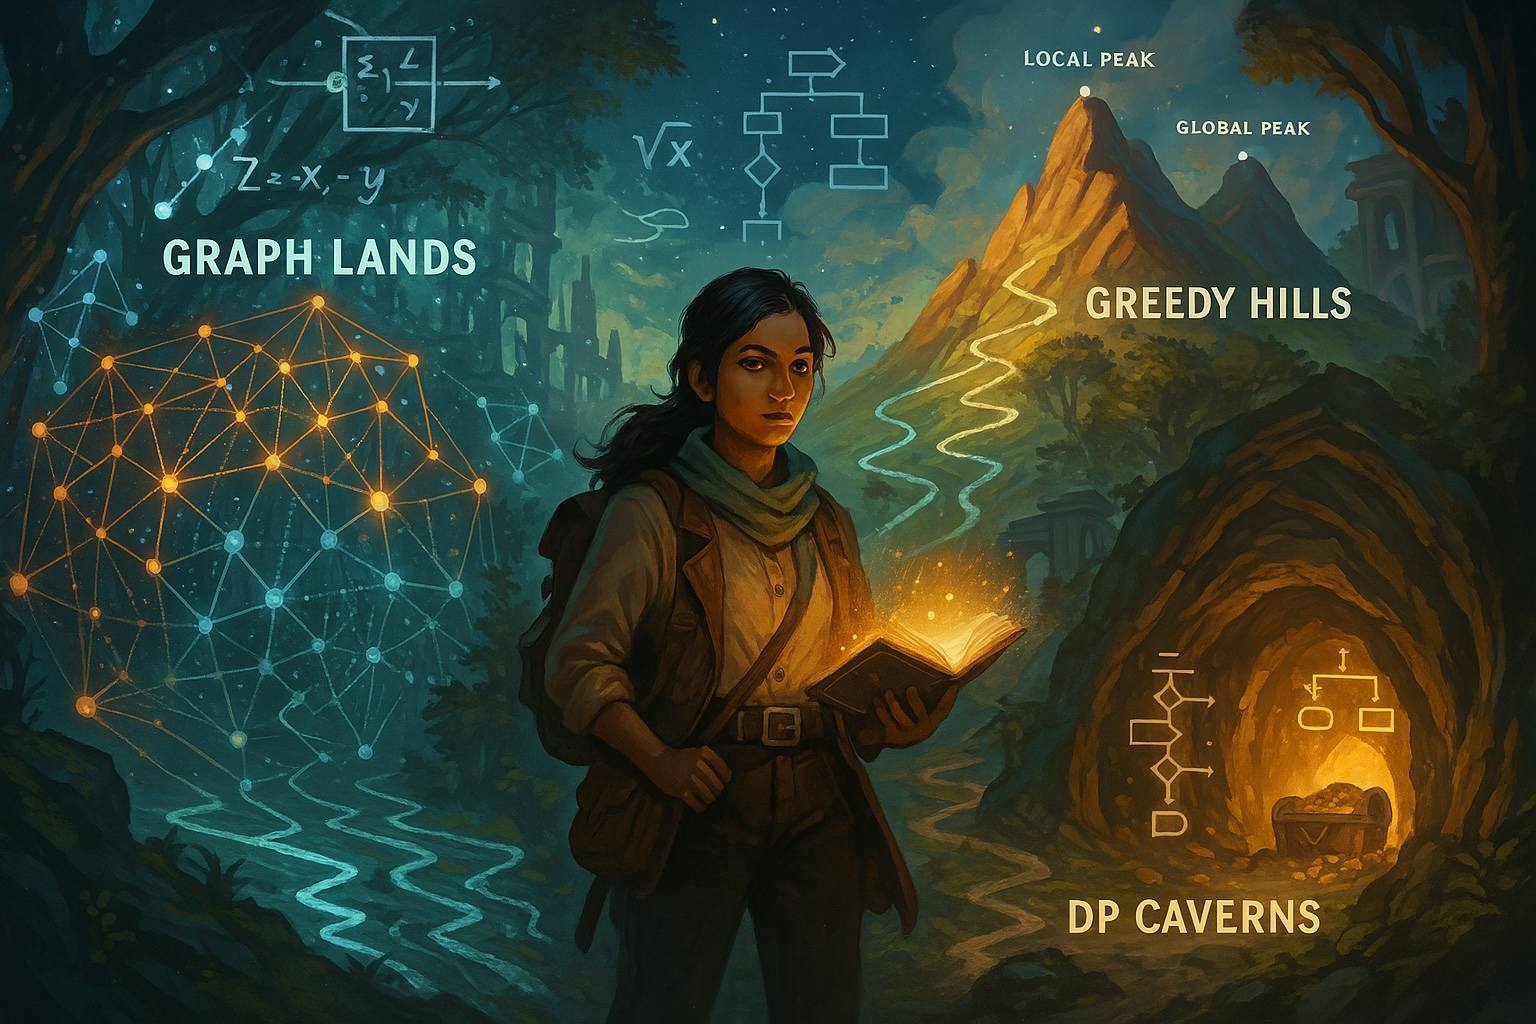
\includegraphics[trim=0 2cm 0 0cm, clip, width=\textwidth]{title}
\begin{questions}
  

\titledquestion{Introduction to Epidemiology}

  You are given a set of nodes representing villages and mountains. Some villages are initially infected, and others are healthy. Villages are connected by undirected paths, which define how the disease can potentially spread. There is a path between any two nodes, but the disease cannot cross a mountain. That is, a mountain is a special type of node through which the disease cannot enter or pass.
  
Each day, the disease spreads from an infected village to its directly connected healthy villages. We are interested to:
\begin{itemize}
\item Visualize the graph.
\item Simulate the spread of the disease over time.
\item Compute the minimum number of days required to infect all reachable healthy villages.
\item Identify the healthy villages that cannot be infected (due to mountain barriers).
\end{itemize}

\heading{Input Format}

The first line of the input contains two integers, $n$ and $m$, the numbers of nodes and edges respectively, where $n-1\le m\le \frac{n(n-1)}{2}$.

The next $m$ lines each contain two integers, $u$ and $v$, indicating an edge between vertex $u$ and vertex $v$ where $0 le u,n < n$.

The next line contains two integers $p$ and $q$, the number of mountains and initially infected villages respectively, where $(1\le p,q \le n)$ and $2\le p+q \le n$.

The next line contains $p$ integers $a_1\ a_2\ a_3\ldots a_p$ where each $0 \le a_i< n$ indicates a mountain.

The next line contains $q$ integers $b_1\ b_2\ b_3\ldots b_q$ where each $0 \le b_j< n$ indicates an initially infected village.

It is guaranteed that $a_i\ne b_j$ for all valid values of $i$ and $j$,

\heading{Output Format}

The first line of the output should contain a single integer denoting the minimum number of days to infect all reachable healthy villages. Output 0 if all reachable villages are already infected.

The second line of the output contains the nodes that represent the healthy villages that cannot be infected. Output 0 if all healthy villages can get infected.

\heading{Sample}
\begin{minipage}{.2\textwidth}
\begin{tabular}{|l|l|}
  \hline
  Input & Output\\\hline
7 6 & 2 \\
1 2 & 5 6 7\\
2 3 & \\
3 4 & \\
4 5 & \\
5 6 & \\
8 7 & \\
1 1 & \\
4 & \\
1 & \\\hline
\end{tabular}
\end{minipage}
\begin{minipage}{.75\textwidth}
The input describes a graph with $n=7$ nodes and $m=6$ edges. The next 6 lines describe the edges. There are $p=1$ mountain nodes and $q=1$ initially infected village nodes. The $p=1$ nodes representing mountains are: $4$. The $q=1$ nodes representing initially infected villages are: $1$.

The output declares a minimum of 2 days for the maximal spread of the disease. On Day 1, the disease spreads from node 1 to node 2. On Day 2, it spreads from node 2 to node 3. It cannot spread further as it is blocked by the mountain at 4. The output declares that the villages $5, 6, 7$ do not get infected.
\end{minipage}

\heading{Tasks}

\begin{parts}
\part[5] Design a linear-time algorithm to simulate the spread. That is, ensure your solution runs in $\mathcal{O}(n + m)$ time, where $n$ is the number of nodes and $m$ is the number of edges. Describe below any considerations, e.g. appropriate data structures, to ensure the linear run time.
  \begin{solution}
    
  \end{solution}
\part[5] Submit files, \texttt{disease.in} and \texttt{disease.py}, where the former contains input and the latter reads the input and implements your algorithm on it to produce the output. You may design any reasonable input. 
\part[5] Submit an animation, \texttt{disease.mp4}, which simulates the spread of the disease on your graph from above. The last frame should include the output of your program.
\end{parts}


%\maketitle
\titledquestion{Pakistan Trip Planning}[10]

  For this problem, we will study the road network of Pakistan to construct a graph modeling the roads between at least 12 cities, listed below, and implement an All-Pairs Shortest Path Algorithm (e.g., Floyd-Warshall) to find the shortest road distance between any pair of cities. You will write a program that visualizes the network, and interactively displays the shortest road distance between two input cities.

  The cities include the capital cities of each province/region:
  \begin{itemize}
    \item Islamabad (Capital Territory)
    \item Lahore (Punjab)
    \item Karachi (Sindh)
    \item Peshawar (Khyber Pakhtunkhwa)
    \item Quetta (Balochistan)
    \item Muzaffarabad (Azad Jammu \& Kashmir)
    \item Gilgit (Gilgit-Baltistan)
    \item At least five other major cities of your choice.
  \end{itemize}

  \begin{parts}
  \part[5] Submit a file, \texttt{roads.py}, that hard codes the graph, visualizes it, applies your chosen all-pairs shortest path algorithm on it and stores the distances, and handles interactive queries (case-insensitive and handling invalid input).
  \part[5] Include below any notes on your approach, cities used, and assumptions.
    \begin{solution}
      
    \end{solution}
  \part[5] Submit a short demo video (no longer than 5 minutes), \texttt{roads.mp4}, of a run of your program. The video should include the graph visualization, interaction with the user, and commentary by you including details of the algorithm, visualization, and interaction. Make sure that the visualization highlights any selected shortest route.
  \end{parts}


\titledquestion{Greedy Bucket}

  Figure \ref{fig:bucket} presents the Bucket Algorithm (Algorithm A) and illustrates a few steps of its dry run on an unweighted and undirected graph in which the bucket is represented by the purple colored area. The algorithm appears to useful to detect connected components in the graph. However, with slight modifications, it can do a lot more!

  Figure \ref{fig:bucketspan} presents Algorithm B which modifies Algorithm A to output a tree containing connected vertices. Such a tree is called the \textit{spanning tree}. Formally, ``a spanning tree $T$ of an undirected graph $G$ is a subgraph that is a tree which includes all of the vertices of $G$. In general, a graph may have several spanning trees, but a graph that is not connected will not contain a spanning tree $\ldots$ [rather a] spanning forest.''\footnote{\url{https://en.wikipedia.org/wiki/Spanning_tree}}
  
  \begin{figure}
    \begin{center}
    \begin{minipage}{.8\textwidth}
    \textbf{Algorithm A: The Bucket Algorithm}\\
    \underline{Input:} Graph $G = (V, E)$\\
    \underline{Output:} Bucket $B \subseteq V$ (a set of vertices)

    \begin{enumerate}
    \item Choose any vertex $x \in V$
    \item Initialize Bucket $B \leftarrow x$
    \item While there exists an edge $(u, v) \in E$ such that $u \in B$ and $v \not\in B$:
      \begin{enumerate}
      \item Add vertex $v$ to $B$
      \end{enumerate}
    \end{enumerate}
  \end{minipage}\\[5pt]

    \rule{300pt}{.5pt}\\
    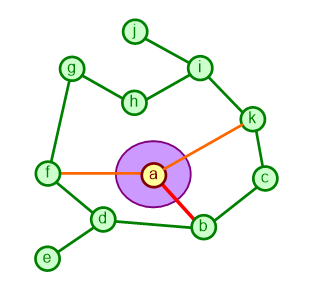
\includegraphics[scale=0.6]{a}
    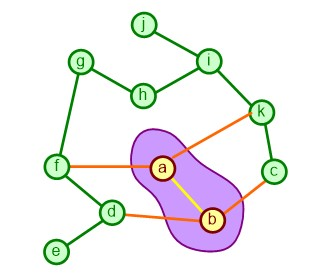
\includegraphics[scale=0.6]{b}
    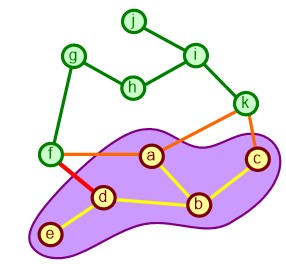
\includegraphics[scale=0.6]{c}
    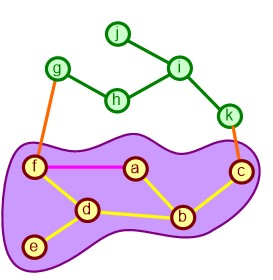
\includegraphics[scale=0.6]{d}      
  \end{center}
  \caption{The bucket algorithm (top) and a visualization (bottom) of a run of the algorithm on an unweighted and undirected graph. The \textit{bucket} is represented by the purple colored area. It expands from one step to the next.}
    \label{fig:bucket}
  \end{figure}
  \begin{figure}
    \begin{center}
    \begin{minipage}{.8\textwidth}
\textbf{Algorithm B: Bucket Algorithm with Spanning Tree}\\
\underline{Input:} Graph $G = (V, E)$ represented as an adjacency matrix\\
\underline{Output:} Spanning tree $T$

\begin{enumerate}
    \item Choose any vertex $x \in V$
    \item Initialize Bucket $B \leftarrow x$, Tree $T \leftarrow \emptyset$
    \item While there exists an edge $(u, v) \in E$ such that $u \in B$ and $v \not\in B$:
    \begin{enumerate}
        \item Add vertex $v$ to $B$
        \item Add edge $(u, v)$ to $T$
    \end{enumerate}
    \item Return $T$
\end{enumerate}      
    \end{minipage}
  \end{center}
  \caption{The bucket algorithm from Figure \ref{fig:bucket} is modified to compute a spanning tree.}
    \label{fig:bucketspan}
  \end{figure}

  \begin{parts}
  \part[5]  Modify Algorithm B to operate on a \textit{weighted} undirected graph and output its Minimum Spanning Tree i.e. a spanning tree that connects all the vertices with the least possible sum of edge weights. Call this Algorithm C.\\
    Hint: be greedy in step 3b).
    \begin{solution}
      
    \end{solution}
  \part[5] For Algorithm C that you developed above, visualize its run on the graph below starting from vertex $a$. Highlight the bucket and the minimum spanning tree edges at every step to clearly show how they grow (as shown in the sample dry run for Algorithm A).
    \begin{solution}\null\\
    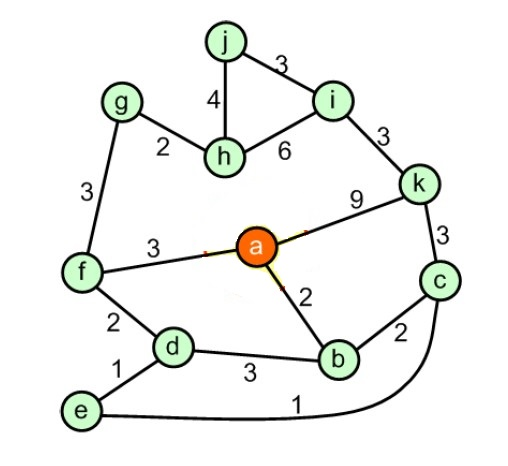
\includegraphics[scale=0.4]{e}
    \end{solution}
  \part[5] Derive the time complexity of Algorithm C.
    \begin{solution}

    \end{solution}
  \part[5] Now let’s design another algorithm, where now we \textit{remove} certain edges frmo $G$ such that the resulting graph is a Minimum Spanning Tree. Let’s call this Algorithm D.\\
    Note that while removing edges, we need to make sure the graph stays connected! To check connectivity use Algorithm A.
    \begin{solution}
      
    \end{solution}
  \part[5] For Algorithm D that you developed above, visualize its run on the graph below starting from vertex $a$. Highlight the edges you are deleting at every step to clearly show how the graph shrinks into an MST.
    \begin{solution}\null\\
    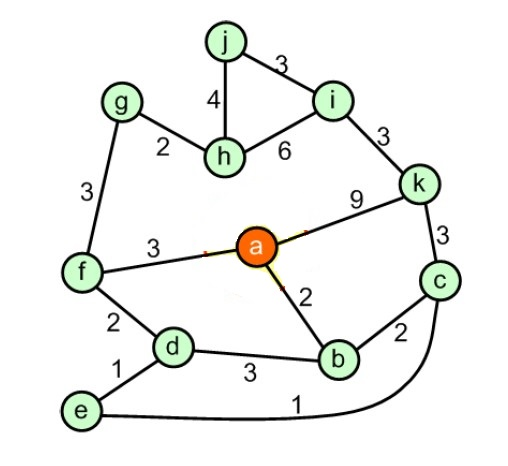
\includegraphics[scale=0.4]{e}
    \end{solution}For Algorithm D that you’ve designed in part c), dry run it on the graph below. 
  \part[5] Derive the time complexity of Algorithm D.
    \begin{solution}
      
    \end{solution}
  \part[5]  Modify Algorithm B to output its \textit{Shortest Path Spanning Tree}. Unlike Minimum Spanning Tree (which minimizes the total weight of the tree), the Shortest Path Spanning Tree focuses on minimizing the distance from the root/starting vertex to each vertex.\\
    Hint: be greedy in step 3b). Call this Algorithm E.
    \begin{solution}
      
    \end{solution}
  \part For Algorithm E that you developed above, visualize its run on the graph below starting from vertex $a$. Highlight the bucket and the shortest path spanning tree edges at every step to clearly show how they grow (as shown in the sample dry run for Algorithm A).
    \begin{solution}\null\\
    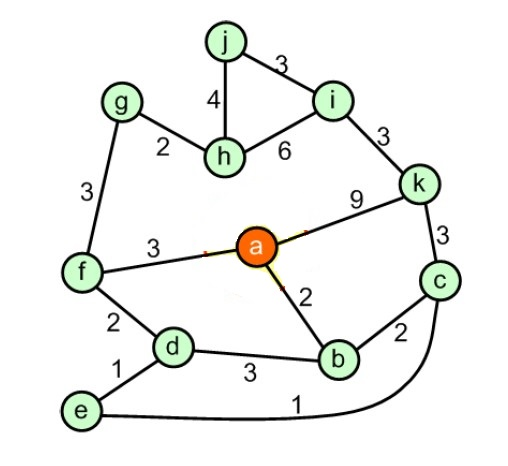
\includegraphics[scale=0.4]{e}
    \end{solution}
  \part Derive the time complexity of Algorithm E.
    \begin{solution}
      
    \end{solution}
\end{parts}


\titledquestion{Getting into Agritech}

  You have deployed a drone to inspect your vast farmlands. A drone's optimal flight distance between recharges is $1000$m. That is flying $x$m induces stress damage (battery overcharge or motor overheat) equal to $(1000-x)^2$.

  You are given a list of distances (in m) to charging stations at increasing distances from the starting point. The distance are given in sorted order. That is, the drone starts at distance $0$ and encounters $n$ charging stations at distances of $a_1 < a_2 < \cdots < a_n$ where each $a_i$ is measured from the starting point. The drone can only stop and recharge at a charging station. It may stop at the charging stations in any order and need not stop at every station but must conclude at the final charging station (at distance $a_n$) which also houses the data center where the drone's recorded data is copied and analyzed.

  As the resident computer scientist, it has come to you to plan the drone's journey.
\begin{parts}
\part[5] Provide a recursive definition of the minimum stress damage. Make sure to indicate the base case. Clearly define any notation that you introduce.
  \begin{solution}
    
  \end{solution}
\part[5] Include a below a visualization of the problem subgraph for $n=5$.
  \begin{solution}
    
  \end{solution}
\part[5] Discuss the time complexity of the solution.
  \begin{solution}
    
  \end{solution}
\part[5] Provide a bottom-up implementation (pseudocode) to compute the minimum stress damage.
  \begin{solution}
    
  \end{solution}
\part[5] Show how the pseudocode can be modified to also compute the sequence of visited charging stations.
  \begin{solution}
    
  \end{solution}
 
\end{parts}

\end{questions}

\end{document}

%%% Local Variables:
%%% mode: latex
%%% TeX-master: t
%%% End:
